
\documentclass[11pt, journal]{IEEEtran}


\usepackage{graphicx}


%% this is to get centered captions (figure)
\makeatletter
\long\def\@makecaption#1#2{\ifx\@captype\@IEEEtablestring%
\footnotesize\begin{center}{\normalfont\footnotesize #1}\\
{\normalfont\footnotesize\scshape #2}\end{center}%
\@IEEEtablecaptionsepspace
\else
\@IEEEfigurecaptionsepspace
\setbox\@tempboxa\hbox{\normalfont\footnotesize {#1.}~~ #2}%
\ifdim \wd\@tempboxa >\hsize%
\setbox\@tempboxa\hbox{\normalfont\footnotesize {#1.}~~ }%
\parbox[t]{\hsize}{\normalfont\footnotesize \noindent\unhbox\@tempboxa#2}%
\else
\hbox to\hsize{\normalfont\footnotesize\hfil\box\@tempboxa\hfil}\fi\fi}
\makeatother



% *** CITATION PACKAGES ***
%
\usepackage{cite}



% *** GRAPHICS RELATED PACKAGES ***
%
\ifCLASSINFOpdf
  \usepackage[pdftex]{graphicx}

\else

\fi



% *** SUBFIGURE PACKAGES ***
\usepackage[tight,footnotesize]{subfigure}


% *** PDF, URL AND HYPERLINK PACKAGES ***
%
\usepackage{url}


% correct bad hyphenation here
\hyphenation{op-tical net-works semi-conduc-tor}

\begin{document}
%
% paper title
% can use linebreaks \\ within to get better formatting as desired
\title{Analysis of Ufo Sightings}


\author{ \parbox{3 in}{\centering Anna Bussas bussas@mail.hs-ulm.de\\
Syndey Nkemakolam nkemakolam@mail.hs-ulm.de\\
Kasparas Gudzius gudzius@mail.hs-ulm.de\\
Zhiwen Lian lian@mail.hs-ulm.de\\
Tim Hutttlestone huttlestone@mail.hs-ulm.de\\
				 University of Applied Sciences Ulm\\
 %        {\tt\small {goldstein}@hs-ulm.de}}
 }
}


% The paper headers
\markboth{ }{A Template Paper}




% make the title area
\maketitle

%%%%%%%%%%%%%%%%%%%%%%%%%%%%%%%%%%%%%%%%%%%%%%%%%%%%%%%%%%%%%%%%%%%%%%%%%%%%%%%%%%%%%%%%%%%%%%%%%%%%%%%%%%%%%%%%%%%%%%%%%%%%%%%%
%%%%%%%%%%%%%%%%%%%%%%%%%%%%%%%%%%%%%%%%%%%%%%%%%%%%%%%%%%%%%%%%%%%%%%%%%%%%%%%%%%%%%%%%%%%%%%%%%%%%%%%%%%%%%%%%%%%%%%%%%%%%%%%%
\begin{abstract}
Based on the data resourse from kaggle.com and the data processing by CRISP-DM, we can observe that most people saw UFOs as a light shape in the US during Summer in 2011. 
\end{abstract}


%%%%%%%%%%%%%%%%%%%%%%%%%%%%%%%%%%%%%%%%%%%%%%%%%%%%%%%%%%%%%%%%%%%%%%%%%%%%%%%%%%%%%%%%%%%%%%%%%%%%%%%%%%%%%%%%%%%%%%%%%%%%%%%%
%%%%%%%%%%%%%%%%%%%%%%%%%%%%%%%%%%%%%%%%%%%%%%%%%%%%%%%%%%%%%%%%%%%%%%%%%%%%%%%%%%%%%%%%%%%%%%%%%%%%%%%%%%%%%%%%%%%%%%%%%%%%%%%%
\section{Introduction}
\label{sec:intro}
We want to analyse the database ufo sightings from
the website kaggle.com. For this we want to figure out 
when and where the UFOs show up mostly and how they look like. 
\subsection{Scenario} \label{subsec:scenario}
The data source has in total 11 columns which covers the discovering time, location, shapes, duration and so on. As our goal is to find out the shapes, country and the number of ufo sightings depending on daytime or nighttime, we need to create a data warehouse containing at least, the information of shapes, country, time category.

\subsection{Structure of the Paper} \label{subsec:struct}
The paper is structured as follows: in Section~\ref{sec:dataunderstanding} we present the availability of Open Data we used in this project.
Then, in Section~\ref{sec:concept} we describe what is our concern to model the original data to our expected data. Finally, we conclude our work in Section~\ref{sec:concl} with (XXXXXXXXXX placeholder --> to see if any section we want to add).
In Section ~\ref{sec:dataPreparation}, ~\ref{sec:modeling},~\ref{sec:Evaluation}, we will introduce how we process the data under CRISP-DM.


%%%%%%%%%%%%%%%%%%%%%%%%%%%%%%%%%%%%%%%%%%%%%%%%%%%%%%%%%%%%%%%%%%%%%%%%%%%%%%%%%%%%%%%%%%%%%%%%%%%%%%%%%%%%%%%%%%%%%%%%%%%%%%%%
\section{Open Data: UFO Sightings} \label{sec:dataunderstanding}
As part of the \emph{Data Understanding} phase for our data science project, we first look at the state concerning our problem. The material presented in this section is based on Kaggle \cite{kaggle}.

%%%%%%%%%%%%%%%%%%%%%%%%%%%%%%%%%%%%%%%%%%%%%%%%%%%%%%%%%%%%%%%%%%%%%%%%%%%%%%%%%%%%%%%%%%%%%%%%%%%%%%%%%%%%%%%%%%%%%%%%%%%%%%%%
\section{Concept for Problem} \label{sec:concept}
During the \emph{Data Understanding} phase, we find out a problem that we don't directly have the data we need .Additionally, some entries have NULL values. Accordingly, we need to have our Data prepared before the Analysis.

\subsection{Data Profiling}\label{subsec:dataProfiling}
In the \emph{Data Profiling} step, we realise we do not need to keep some columns. Accordingly, we will only keep the following columns:
\begin{itemize}
    \item datetime
    \item city
    \item state
    \item country
    \item shape
    \item duration(second)
    \item date posted
\end{itemize}
Also, for the NULL values, we will fill a necessary value in different columns:
\begin{itemize}
    \item city / state / country\\
    If there are NULL values in city or state but not country. We will fill in the country in those two columns because we will mainly focus on the fact that the sighting was in a specific country. For those with both state and country missing, we will try to look at the city name, find the country and manually map as accurately as possible. The rest without enough information were filled with "unknown".
    \item shape\\
    We will fill in "unknown" to replace the NULL values.
\end{itemize}

\subsection{Tools}\label{subsec:tools}
The list of all tools we use in this project and the purpose:  
\begin{itemize}
    \item SQLiteManager\\
    Data Cleaning, ETL process, CDWH \& DM creation
    \item DBSchema\\
    Forward Engineering
    \item BIRT\\
    Analytics
    \item Python\\
    Data Cleaning
\end{itemize}
    
\subsection{DWH layout}\label{subsec:DWHLayout}
After the ELT process, we should have a DHW which looks like this:
\begin{figure}[htb]
	\centering
		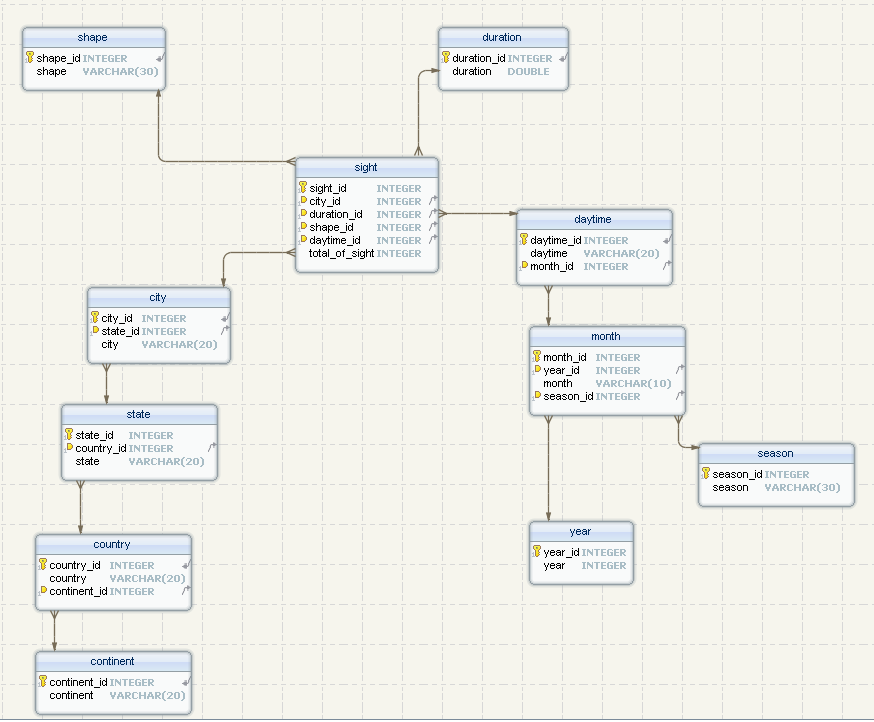
\includegraphics[width=1.0\columnwidth]{images/CDWHUFO}
	\caption{DWH layout}
	\label{fig:CDWHlayout}
\end{figure}

 
%%%%%%%%%%%%%%%%%%%%%%%%%%%%%%%%%%%%%%%%%%%%%%%%%%%%%%%%%%%%%%%%%%%%%%%%%%%%%%%%%%%%%%%%%%%%%%%%%%%%%%%%%%%%%%%%%%%%%%%%%%%%%%%%
%%%%%%%%%%%%%%%%%%%%%%%%%%%%%%%%%%%%%%%%%%%%%%%%%%%%%%%%%%%%%%%%%%%%%%%%%%%%%%%%%%%%%%%%%%%%%%%%%%%%%%%%%%%%%%%%%%%%%%%%%%%%%%%%
\section{Data Preparation} \label{sec:dataPreparation}
This section deals with the implementation of the concept described in Section~\ref{sec:concept} following the \emph{Data Preparation}
phase of CRISP-DM. 

To solve the problem, we have the following steps:
\begin{itemize}
  \item step 1 Extract \\
  Download the data from the website then create a database to store all raw data.
  \item step 2 Filtering\\
  Fill in values by the rule that was mentioned in \ref{subsec:dataProfiling}.
  \item step 3 Enrichment\\
  We would like to see some relationship between the sighting, season, daytime or nighttime, country and so on.In other words, we need different dimentions. So we will create "new" data by using algorithms:
  \begin{itemize}
      \item Create new columns for the year, month, day, hour, daytime, season
      \item Column year, month, day,hour\\
      Extract data from column datetime
      \item Column daytime\\
      From 6am to 6pm, it is defined as daytime. The rest is defined as nighttime
      \item Column season\\
      Compute by column month
  \end{itemize}
  
\end{itemize}

%%%%%%%%%%%%%%%%%%%%%%%%%%%%%%%%%%%%%%%%%%%%%%%%%%%%%%%%%%%%%%%%%%%%%%%%%%%%%%%%%%%%%%%%%%%%%%%%%%%%%%%%%%%%%%%%%%%%%%%%%%%%%%%%
\section{Modeling} \label{sec:modeling}
This section is to analyse the data we have prepared from Section ~\ref{sec:dataPreparation}.

To analyse, we have the following steps:
\begin{itemize}
    \item step 1\\
    Import Cleaning Data in DWH (see DWH Layout in ~\ref{subsec:DWHLayout})
    \item step 2\\
    For the performance and speed, we created four data marts for our goal (See Fig. \ref{fig:dm-cms}, \ref{fig:dm-css}, \ref{fig:dm-dcd}, \ref{fig:dm-scy})
      
    \begin{figure}[htb]
        \centering
            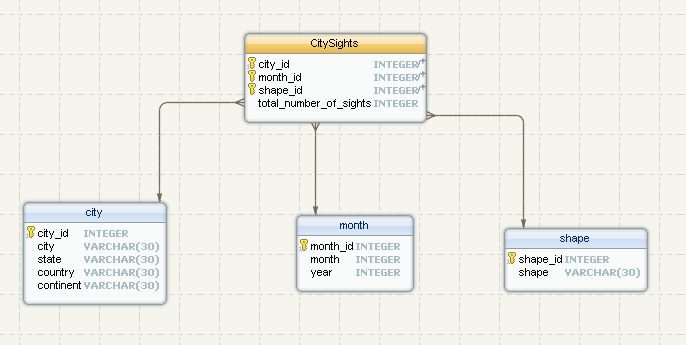
\includegraphics[width=1.0\columnwidth]{images/city-month-shape}
        \caption{Data mart - city/month/shape}
        \label{fig:dm-cms}
    \end{figure}

     \begin{figure}[htb]
            \centering
	            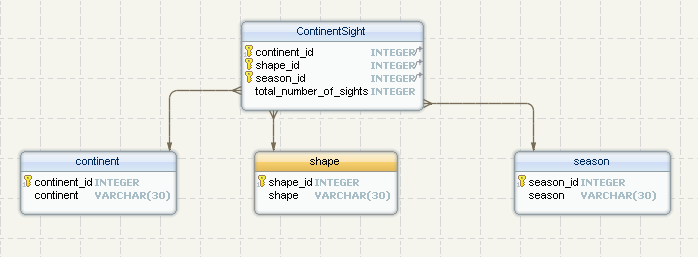
\includegraphics[width=1.0\columnwidth]{images/continent-shape-season}
            \caption{Data mart - continent/shape/season}
            \label{fig:dm-css}
        \end{figure}

     \begin{figure}[htb]
        \centering
            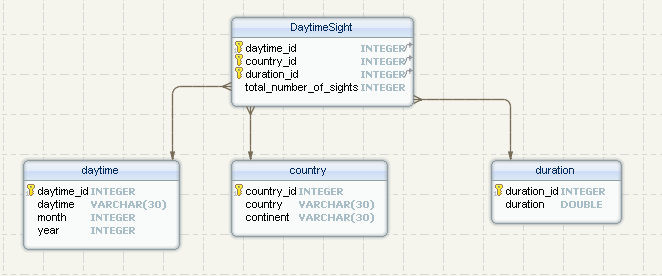
\includegraphics[width=1.0\columnwidth]{images/daytime-country-duration}
        \caption{Data mart - daytime/country/duration}
        \label{fig:dm-dcd}
    \end{figure}

     \begin{figure}[htb]
        \centering
            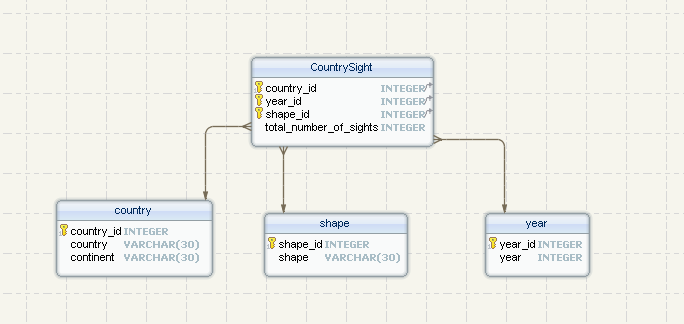
\includegraphics[width=1.0\columnwidth]{images/shape-country-year}
        \caption{Data mart - shape/country/year}
        \label{fig:dm-scy}
    \end{figure}
        
    \item step 3
    Using BIRT, we generated reports and found the following facts:
        \begin{itemize}
            \item Number of sightings in North American is extremely higher than in other continents. The next continent with the highest number of sightings is Europe.(See Fig.\ref{fig:continent})\\
            - Data mart - Shape/Country/Year\\
            - Data cube - continent
                
            \item Nearly all sightings were in the US.(See Fig. \ref{fig:country})\\
            - Data mart - Shape/Country/Year\\
            - Data cube - contry
               
            \item The most Sightings were seen in 2011. We can see that it obviously increased between the years 1995 and 2011.(See Fig. \ref{fig:year} )\\
            - Data mart - Shape/Country/Year\\
            - Data cube - year
                
            \item UFOs are most seen during the Summer. (See Fig. \ref{fig:sight-season})\\
            - Data set - data mart - Continent/Shape/Season\\
            - Data cube - season
                 
            \item Different UFO shapes are seen and the most common was light.(See Fig. \ref{fig:shape})\\
            - Data set - data mart - Continent/Shape/Season\\
            - Data cube - shape
                
            \item In different continents, the most seen shape was also light. (See Fig. \ref{fig:shape-continent})\\
            - Data set - data mart - Continent/Shape/Season\\
            - Data cube - shape,continent
                
            \item In each season, light shape was also the most common. (See Fig. \ref{fig:shape-season})\\
            - Data set - data mart - Continent/shape/season\\
            - Data cube - season, shape
                
        \end{itemize}
        \begin{figure}[htb]
            \centering
                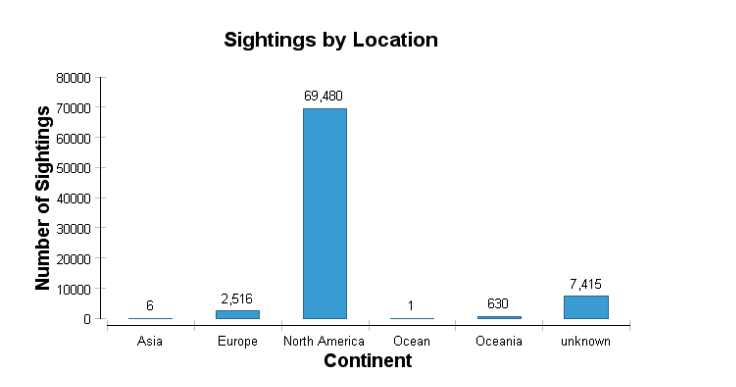
\includegraphics[width=1.0\columnwidth]{images/continent}
            \caption{Sightings by Location - Continent}
            \label{fig:continent}
        \end{figure}
        \begin{figure}[htb]
            \centering
                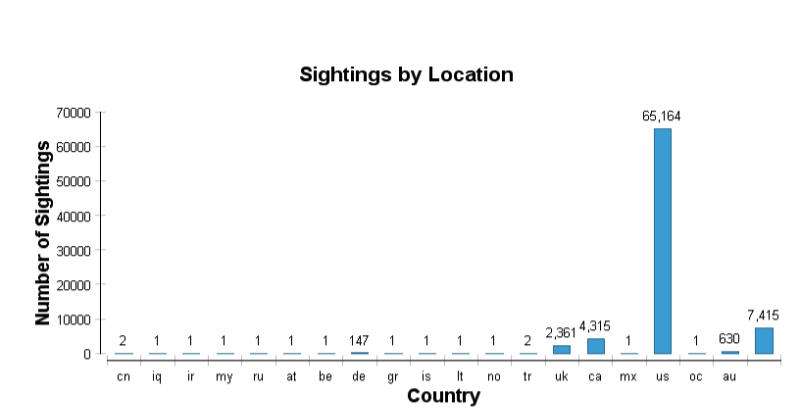
\includegraphics[width=1.0\columnwidth]{images/country}
            \caption{Sightings by Location - country}
            \label{fig:country}
        \end{figure}
        \begin{figure}[htb]
            \centering
                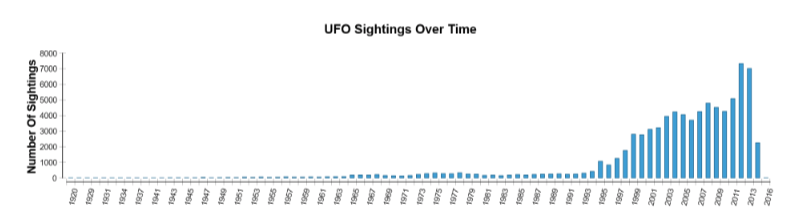
\includegraphics[width=1.0\columnwidth]{images/year}
            \caption{Sightings Over Time}
            \label{fig:year}
        \end{figure}
        \begin{figure}[htb]
            \centering
                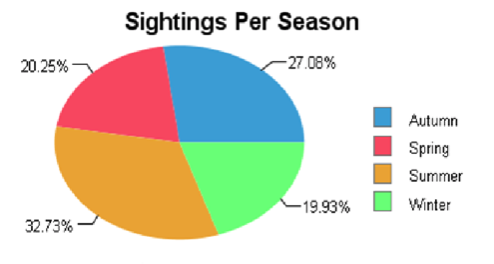
\includegraphics[width=1.0\columnwidth]{images/sightings-season}
            \caption{Sightings Per Season}
            \label{fig:sight-season}
        \end{figure}
        \begin{figure}[htb]
            \centering
                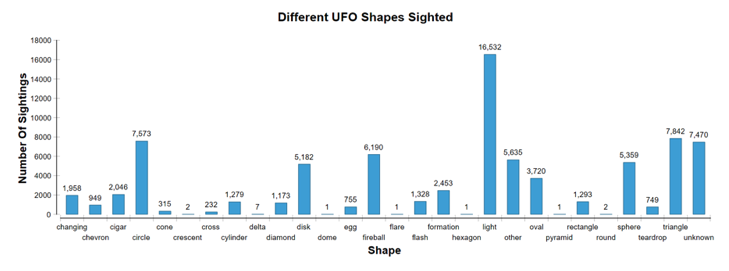
\includegraphics[width=1.0\columnwidth]{images/shape}
            \caption{Different UFO Shapes Sighted}
            \label{fig:shape}
        \end{figure}
        \begin{figure}[htb]
            \centering
                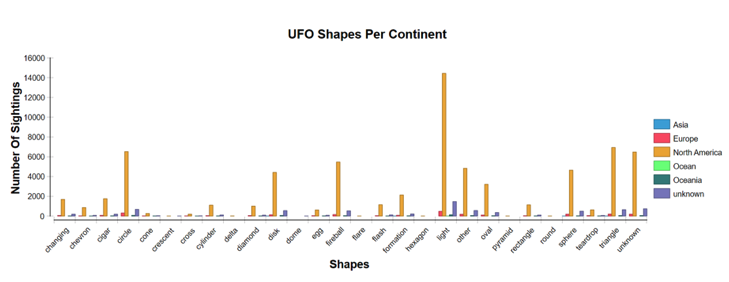
\includegraphics[width=1.0\columnwidth]{images/shape-continent}
            \caption{Shapes Per Continent}
            \label{fig:shape-continent}
        \end{figure}
        \begin{figure}[htb]
            \centering
                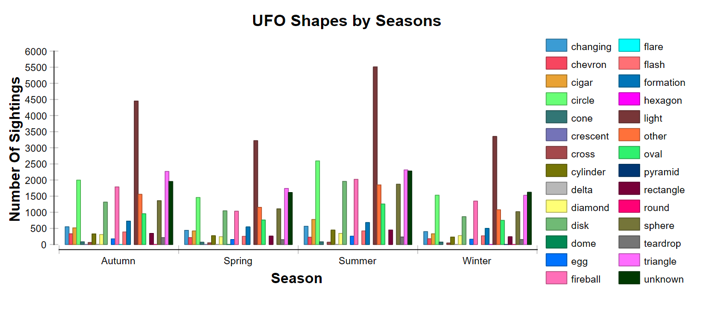
\includegraphics[width=1.0\columnwidth]{images/shapes-seasons}
            \caption{Shapes Per Seasons}
            \label{fig:shape-season}
        \end{figure}
\end{itemize}


%%%%%%%%%%%%%%%%%%%%%%%%%%%%%%%%%%%%%%%%%%%%%%%%%%%%%%%%%%%%%%%%%%%%%%%%%%%%%%%%%%%%%%%%%%%%%%%%%%%%%%%%%%%%%%%%%%%%%%%%%%%%%%%%
\section{Evaluation} \label{sec:Evaluation}
From the reports, we can find out the number of shapes, country and the number of ufo sightings depending on daytime or nighttime. Also the reports in different dimentions. We can safely say that we have reached the goal after evaluation.

%%%%%%%%%%%%%%%%%%%%%%%%%%%%%%%%%%%%%%%%%%%%%%%%%%%%%%%%%%%%%%%%%%%%%%%%%%%%%%%%%%%%%%%%%%%%%%%%%%%%%%%%%%%%%%%%%%%%%%%%%%%%%%%%
\section{Conclusion} \label{sec:concl}
We have shown in this paper how we processed the data under CRISP-DM and it shows different dimentions of shape, continents, country, seasons. 

%%%%%%%%%%%%%%%%%%%%%%%%%%%%%%%%%%%%%%%%%%%%%%%%%%%%%%%%%%%%%%%%%%%%%%%%%%%%%%%%%%%%%%%%%%%%%%%%%%%%%%%%%%%%%%%%%%%%%%%%%%%%%%%%
%%%%%%%%%%%%%%%%%%%%%%%%%%%%%%%%%%%%%%%%%%%%%%%%%%%%%%%%%%%%%%%%%%%%%%%%%%%%%%%%%%%%%%%%%%%%%%%%%%%%%%%%%%%%%%%%%%%%%%%%%%%%%%%%
% see file Literatur/bibliography!
\bibliographystyle{plaindin}
\bibliography{bibliography}

\end{document}
